\documentclass{beamer}
% Use DS9 global theme (includes pgfplots for visualization)
\usepackage{../../../../latex-beamer/shared/templates/ds9_theme}

% Title page configuration
\title[Friction, Drag, and Elasticity]{PHYS12 CH: 5.1, 5.2, and 5.3}
\subtitle{Further Applications of Newton's Laws}
\author[Mr. Gullo]{Mr. Gullo}
\date[Fall 2025]{September 17, 2025}

\begin{document}
\frame{\titlepage}

\begin{frame}
\frametitle{Learning Objectives}
\begin{itemize}
    \item By the end of this lesson, you will be able to: \pause
    \item \textbf{Friction (5.1)}
    \begin{itemize}
        \item Discuss the general characteristics of friction. \pause
        \item Describe static vs. kinetic friction. \pause
        \item Calculate the magnitude of static and kinetic friction.
    \end{itemize} \pause
    \item \textbf{Drag Forces (5.2)}
    \begin{itemize}
        \item Express the drag force mathematically. \pause
        \item Define and determine terminal velocity.
    \end{itemize} \pause
    \item \textbf{Elasticity (5.3)}
    \begin{itemize}
        \item State Hooke's law and explain it using stress and strain. \pause
        \item Describe Young's modulus, shear modulus, and bulk modulus. \pause
        \item Determine the change in length of an object under tension or compression.
    \end{itemize}
\end{itemize}
\end{frame}

\begin{frame}
\frametitle{Building on Physics 11}
\begin{block}{Review from Physics 11}
\begin{itemize}
    \item The model for static friction ($f_s \leq \mu_s N$) and kinetic friction ($f_k = \mu_k N$). \pause
    \item Applying friction forces to problems, especially on inclined planes. \pause
    \item Hooke's Law ($F = kx$) for ideal springs.
\end{itemize}
\end{block} \pause

\begin{block}{New Concepts in Physics 12}
\begin{itemize}
    \item \textbf{Drag Forces}: Introducing forces that depend on velocity ($F_D \propto v^2$). \pause
    \item \textbf{Elasticity}: A deeper look at material properties using Stress and Strain. \pause
    \item \textbf{Terminal Velocity}: The concept of a maximum speed in freefall when drag balances gravity.
\end{itemize}
\end{block}
\end{frame}

\section{5.1 Friction}

\begin{frame}
\frametitle{Key Concepts: Friction}
\begin{itemize}
    \item Friction is a force that opposes relative motion or attempted motion between surfaces in contact. \pause
    \item It acts parallel to the surface. \pause
    \item There are two main types:
    \begin{description}
        \item[Static Friction ($f_s$)] Acts on stationary objects. It is a \alert{responsive force} that matches the applied force up to a maximum value. \pause
        \item[Kinetic Friction ($f_k$)] Acts on moving objects. It is generally a constant value for a given speed and is \alert{less than} the maximum static friction.
    \end{description}
\end{itemize}
\end{frame}

\begin{frame}
\frametitle{Essential Equations: Friction}
\begin{alertblock}{Static Friction}
The magnitude of static friction $f_s$ can have any value up to a maximum:
\[ f_s \leq \mu_s N \]
where $\mu_s$ is the coefficient of static friction and $N$ is the normal force. Motion begins when the applied force exceeds $f_{s(\text{max})} = \mu_s N$.
\end{alertblock} \pause

\begin{exampleblock}{Kinetic Friction}
Once an object is moving, the friction force is kinetic friction:
\[ f_k = \mu_k N \]
where $\mu_k$ is the coefficient of kinetic friction. Typically, $\mu_k < \mu_s$.
\end{exampleblock}
\end{frame}

\begin{frame}
\frametitle{The Static-Kinetic Friction Threshold}
\begin{center}
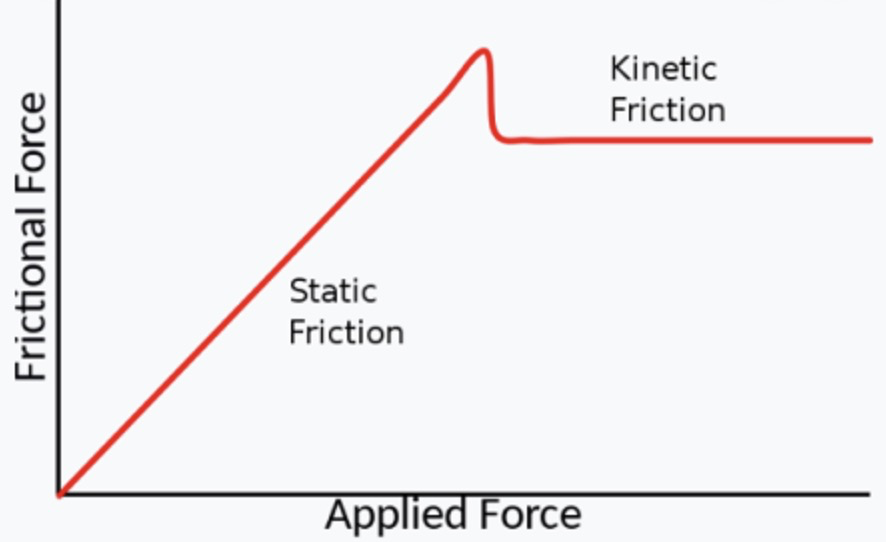
\includegraphics[width=0.6\textwidth]{../images/thresholdstatic-kinetic-friction.png}
\end{center}
\begin{block}{The Activation Energy Threshold}
This graph illustrates the critical transition point where static friction (higher resistance) gives way to kinetic friction (lower resistance). The ``drop'' represents the activation energy needed to overcome the initial barrier -- once this threshold is crossed, motion becomes sustained with less effort.
\end{block}
\end{frame}

\begin{frame}
\frametitle{Video Activity: The 5-Second Rule}
\begin{alertblock}{Motivational Video Prompt}
Watch \textbf{How to Stop Screwing Yourself Over} by Mel Robbins (TEDxSF)
\begin{itemize}
    \item \textbf{Time segment}: 9:00 - 13:30
    \item Focus on: The science behind activation energy and taking action
    \item Connect to: How this relates to overcoming static friction in physics
\end{itemize}
\end{alertblock}

\begin{exampleblock}{The 5-Second Rule}
\textbf{If you have an impulse to act on a goal, you must physically move within 5 seconds or your brain will kill the idea.} This countdown creates the activation energy needed to overcome static friction and get started.
\end{exampleblock}

\end{frame}

\begin{frame}
\frametitle{Life Lesson: The Threshold of Getting Started}
\begin{alertblock}{The Physics of Procrastination}
The relationship $\mu_k < \mu_s$ teaches us a profound lesson about human behavior:
\begin{itemize}
    \item \textbf{Static friction ($\mu_s$)}: The resistance to starting something new
    \begin{itemize}
        \item Starting a new project, habit, or exercise routine
        \item The initial effort feels much harder than maintaining momentum
        \item This is why "getting started" is often the hardest part
    \end{itemize} \pause
    \item \textbf{Kinetic friction ($\mu_k$)}: The resistance once you're already moving
    \begin{itemize}
        \item Continuing an established habit or routine
        \item Much easier to maintain once you've overcome the initial threshold
        \item Momentum becomes your ally
    \end{itemize}
\end{itemize}
\end{alertblock} \pause

\begin{exampleblock}{Application to Life}
Just like objects in motion tend to stay in motion, people in motion tend to stay in motion. The key is applying enough initial force to overcome static friction -- then let momentum carry you forward!
\end{exampleblock}
\end{frame}

\begin{frame}
\frametitle{Concept Visualization Context: Microscopic Friction}
\begin{itemize}
    \item Why does friction exist? \pause
    \item Even surfaces that look smooth to the naked eye are very rough on a microscopic or atomic level. \pause
    \item Friction arises from two main effects:
    \begin{enumerate}
        \item The interlocking of these microscopic hills and valleys. \pause
        \item Adhesive forces between the molecules of the two surfaces.
    \end{enumerate} \pause
    \item The next slide shows a visual representation of this idea.
\end{itemize}
\end{frame}

\begin{frame}
\frametitle{Concept Visualization: Microscopic Friction}
\begin{alertblock}{[Diagram based on Figure 5.2]}
A magnified view of two surfaces in contact.
\begin{itemize}
    \item The surfaces are shown with rough, jagged profiles, even if they seem smooth macroscopically.
    \item The actual points of contact are only at the tips of the highest "peaks".
    \item When a horizontal force is applied, these peaks must either be broken off or lifted over each other for motion to occur.
    \item A larger normal force ($N$) pushes the surfaces together, increasing the contact area and the force required to move them.
\end{itemize}
\end{alertblock}
\end{frame}

\section{5.2 Drag Forces}

\begin{frame}
\frametitle{Key Concepts: Drag Force}
\begin{itemize}
    \item The drag force ($F_D$) is a resistive force that acts on an object moving through a fluid (like air or water). \pause
    \item It always opposes the direction of the object's velocity. \pause
    \item For most large objects at moderate to high speeds, the drag force is proportional to the square of the velocity ($F_D \propto v^2$). \pause
    \item This means drag increases significantly as an object speeds up.
\end{itemize}
\end{frame}

\begin{frame}
\frametitle{Key Concepts: Terminal Velocity}
\begin{itemize}
    \item Consider an object falling from rest (e.g., a skydiver). \pause
    \item Initially, its velocity is zero, so the drag force is zero. The only force is gravity ($F_g = mg$), and it accelerates downwards at $g$. \pause
    \item As velocity increases, the drag force ($F_D$) increases. The net downward force ($F_{net} = mg - F_D$) decreases, so acceleration decreases. \pause
    \item Eventually, the object is moving so fast that the upward drag force becomes equal in magnitude to the downward force of gravity.
    \[ F_D = mg \] \pause
    \item At this point, $F_{net} = 0$, so acceleration is zero. The object stops accelerating and falls at a constant velocity called \alert{terminal velocity ($v_t$)}.
\end{itemize}
\end{frame}

\begin{frame}
\frametitle{Essential Equations: Drag Force}
\begin{alertblock}{Drag Force Equation}
For many objects (cars, baseballs, skydivers), the drag force is given by:
\[ F_D = \frac{1}{2} C \rho A v^2 \]
\begin{itemize}
    \item $C$: Drag coefficient (a dimensionless number based on shape)
    \item $\rho$: Density of the fluid (e.g., air $\approx 1.21$ kg/m$^3$)
    \item $A$: Cross-sectional area of the object facing the fluid
    \item $v$: Speed of the object
\end{itemize}
\end{alertblock} \pause
\begin{exampleblock}{Terminal Velocity Equation}
By setting $F_D = mg$ and solving for $v$, we get terminal velocity:
\[ v_t = \sqrt{\frac{2mg}{C \rho A}} \]
\end{exampleblock}
\end{frame}

\section{5.3 Elasticity}

\begin{frame}
\frametitle{Key Concepts: Stress and Strain}
When a force is applied to a solid object, it can deform (change its shape). \pause
\begin{description}
    \item[Stress] A measure of the applied force per unit area. It quantifies the internal forces within the object.
    \[ \text{Stress} = \frac{F}{A} \quad (\text{Units: N/m}^2 \text{ or Pascals}) \] \pause
    \item[Strain] A measure of the degree of deformation. It is the fractional change in the object's length.
    \[ \text{Strain} = \frac{\Delta L}{L_0} \quad (\text{Unitless}) \] \pause
\end{description}
For small deformations, most materials obey \textbf{Hooke's Law}: Stress is proportional to Strain.
\end{frame}

\begin{frame}
\frametitle{Essential Equations: Elasticity}
\begin{alertblock}{Hooke's Law}
For a spring-like object, the force is proportional to the deformation:
\[ F = k \Delta L \]
where $k$ is the spring constant.
\end{alertblock} \pause

\begin{exampleblock}{Young's Modulus (Y)}
A material property that measures stiffness in response to tension or compression. It is the ratio of stress to strain.
\[ Y = \frac{\text{Stress}}{\text{Strain}} = \frac{F/A}{\Delta L/L_0} \] \pause
This can be rearranged to find the change in length:
\[ \Delta L = \frac{1}{Y} \frac{F}{A} L_0 \]
\end{exampleblock}
\end{frame}

\begin{frame}
\frametitle{Concept Visualization Context: Stress-Strain Curve}
\begin{itemize}
    \item We can plot stress vs. strain to understand a material's behavior. \pause
    \item In the \alert{elastic region}, the material follows Hooke's Law (linear graph) and returns to its original shape when the stress is removed. \pause
    \item If the stress is too large, the material enters the \alert{plastic region}, where it deforms permanently. \pause
    \item At the \alert{fracture point}, the material breaks. \pause
    \item The next slide visualizes this relationship.
\end{itemize}
\end{frame}

\begin{frame}
\frametitle{Concept Visualization: Stress-Strain Curve}
\begin{alertblock}{[Graph based on Figure 5.11: Deformation vs. Applied Force]}
A graph with Deformation ($\Delta L$) on the y-axis and Applied Force ($F$) on the x-axis.
\begin{itemize}
    \item \textbf{Linear Region}: The graph starts as a straight line from the origin. In this region, Hooke's law is obeyed. The material is elastic. \pause
    \item \textbf{Permanent Deformation}: The graph starts to curve. If the force is removed in this region, the object will not return to its original length. \pause
    \item \textbf{Fracture Point}: The graph ends abruptly where the material breaks.
\end{itemize}
\end{alertblock}
\end{frame}

\section{I do, We do, You do}

\begin{frame}
\frametitle{"I Do": Skiing Exercise (Friction)}
\begin{block}{Problem (Example 5.1)}
A skier with a mass of 62 kg is sliding down a snowy slope angled at $25^\circ$. The force of kinetic friction resisting their motion is known to be 45.0 N.
\newline\newline
Find the coefficient of kinetic friction, $\mu_k$, between the skis and the snow.
\end{block}
\begin{center}
\alert{[Free-body diagram of skier on an incline]}
\end{center}
\end{frame}

\begin{frame}
\frametitle{"I Do": Skiing Exercise - G \& U}
\begin{columns}[T]
\column{0.48\textwidth}
\textbf{G - Givens}
\begin{itemize}
    \item Mass, $m = 62$ kg
    \item Angle, $\theta = 25^\circ$
    \item Kinetic friction force, $f_k = 45.0$ N
    \item Acceleration due to gravity, $g = 9.80$ m/s$^2$
\end{itemize}

\column{0.48\textwidth}
\textbf{U - Unknown}
\begin{itemize}
    \item Coefficient of kinetic friction, $\mu_k = ?$
\end{itemize}
\end{columns}
\end{frame}

\begin{frame}
\frametitle{"I Do": Skiing Exercise - E}
\textbf{E - Equation}
\begin{itemize}
    \item Start with the definition of kinetic friction: $f_k = \mu_k N$. \pause
    \item The normal force $N$ on an incline balances the perpendicular component of weight: $N = w_{\perp} = mg \cos\theta$. \pause
    \item Substitute for $N$: $f_k = \mu_k (mg \cos\theta)$. \pause
    \item \textbf{Rearrange} for the unknown, $\mu_k$:
    \[ \mu_k = \frac{f_k}{mg \cos\theta} \]
\end{itemize}
\end{frame}

\begin{frame}
\frametitle{"I Do": Skiing Exercise - S \& S}
\textbf{S - Substitute}
\begin{itemize}
    \item Plug in the known values with their units:
    \[ \mu_k = \frac{45.0 \text{ N}}{(62 \text{ kg})(9.80 \text{ m/s}^2) \cos(25^\circ)} \]
\end{itemize} \pause
\textbf{S - Solve}
\begin{itemize}
    \item Calculate the denominator: $(62)(9.80)(0.9063) \approx 550.5$ N.
    \item $\mu_k = \frac{45.0}{550.5} \approx 0.08174$
    \item Apply significant figures (3 sig figs from 45.0 N and 62 kg):
    \item \boxed{\mu_k = 0.082}
\end{itemize}
\end{frame}

\begin{frame}
\frametitle{"We Do": Terminal Velocity (Drag)}
\begin{block}{Problem (Example 5.2)}
Find the terminal velocity of an 85-kg skydiver falling in a spread-eagle position.
\newline\newline
Estimate the frontal area as $A = 0.70 \text{ m}^2$, the drag coefficient as $C=1.0$, and use the density of air $\rho=1.21 \text{ kg/m}^3$.
\end{block}
\end{frame}

\begin{frame}
\frametitle{"We Do": Terminal Velocity - G \& U}
\begin{columns}[T]
\column{0.48\textwidth}
\textbf{G - Givens}
\begin{itemize}
    \item $m = 85$ kg
    \item $A = 0.70 \text{ m}^2$
    \item $C = 1.0$
    \item $\rho = 1.21 \text{ kg/m}^3$
    \item $g = 9.80$ m/s$^2$
\end{itemize}

\column{0.48\textwidth}
\textbf{U - Unknown}
\begin{itemize}
    \item Terminal velocity, $v_t = ?$
\end{itemize}
\end{columns}
\end{frame}

\begin{frame}
\frametitle{"We Do": Terminal Velocity - E}
\textbf{E - Equation}
\begin{itemize}
    \item What is our starting equation for terminal velocity? \pause
    \[ v_t = \sqrt{\frac{2mg}{C \rho A}} \] \pause
    \item Is any algebraic rearrangement needed? (No) \pause
    \item Now, let's get ready to substitute our values.
\end{itemize}
\end{frame}

\begin{frame}
\frametitle{"We Do": Terminal Velocity - S \& S}
\textbf{S - Substitute}
\begin{itemize}
    \item Let's plug in the numbers together:
    \[ v_t = \sqrt{\frac{2(85 \text{ kg})(9.80 \text{ m/s}^2)}{(1.0)(1.21 \text{ kg/m}^3)(0.70 \text{ m}^2)}} \]
\end{itemize} \pause
\textbf{S - Solve}
\begin{itemize}
    \item Calculate the value inside the square root. What do you get?
    \item Numerator: $2 \times 85 \times 9.80 = 1666$
    \item Denominator: $1.0 \times 1.21 \times 0.70 \approx 0.847$ \pause
    \item $v_t = \sqrt{\frac{1666}{0.847}} = \sqrt{1967} \approx 44.35$ m/s
    \item \boxed{v_t \approx 44 \text{ m/s}}
\end{itemize}
\end{frame}

\begin{frame}
\frametitle{"You Do": Bone Compression (Elasticity)}
\begin{block}{Problem (Example 5.4)}
Calculate the change in length of the upper leg bone (femur) when a 70.0 kg man supports 62.0 kg of his mass on it.
\newline
\begin{itemize}
    \item \textbf{Givens}:
    \item Mass supported, $m = 62.0$ kg
    \item Original length, $L_0 = 40.0$ cm $= 0.400$ m
    \item Radius, $r = 2.00$ cm $= 0.0200$ m
    \item Young's modulus (bone compression), $Y = 9 \times 10^9$ N/m$^2$
\end{itemize}
\vspace{0.3cm}
Use the GUESS method to find the amount the bone shortens, $\Delta L$.
\end{block}
\end{frame}

\begin{frame}
\frametitle{Reading Homework}
\begin{itemize}
    \item Please ensure you read through Sections 5.1, 5.2, and 5.3 in your textbook. \pause
    \item Pay special attention to:
    \begin{itemize}
        \item The table of coefficients of friction (Table 5.1).
        \item The table of drag coefficients for various shapes (Table 5.2).
        \item Stokes' Law for drag at very low speeds.
        \item Shear Modulus and Bulk Modulus concepts.
    \end{itemize} \pause
    \item The concepts discussed in these sections are important for a full understanding and may appear on assessments.
\end{itemize}
\end{frame}

\begin{frame}
\frametitle{Summary}
\begin{itemize}
    \item \textbf{Friction} is a contact force that opposes motion. We distinguish between static ($f_s \le \mu_s N$) and kinetic ($f_k = \mu_k N$) friction. \pause
    \item \textbf{Drag} is a resistive force from a fluid that depends on velocity ($F_D \propto v^2$). This leads to a \textbf{Terminal Velocity} when the drag force balances gravity. \pause
    \item \textbf{Elasticity} describes how objects deform. \textbf{Stress} ($F/A$) is the applied force per area, and \textbf{Strain} ($\Delta L/L_0$) is the resulting fractional deformation. These are related by a material's \textbf{Young's Modulus}, $Y$. \pause
    \item These concepts provide more realistic models for applying Newton's Laws to complex, everyday situations.
\end{itemize}
\end{frame}

\end{document}